\documentclass{standalone}
\usepackage{tikz}
\usetikzlibrary{patterns, positioning}
\usepackage[sfdefault]{ClearSans} %% option 'sfdefault' activates Clear Sans as the default text font
\usepackage[T1]{fontenc}

\begin{document}
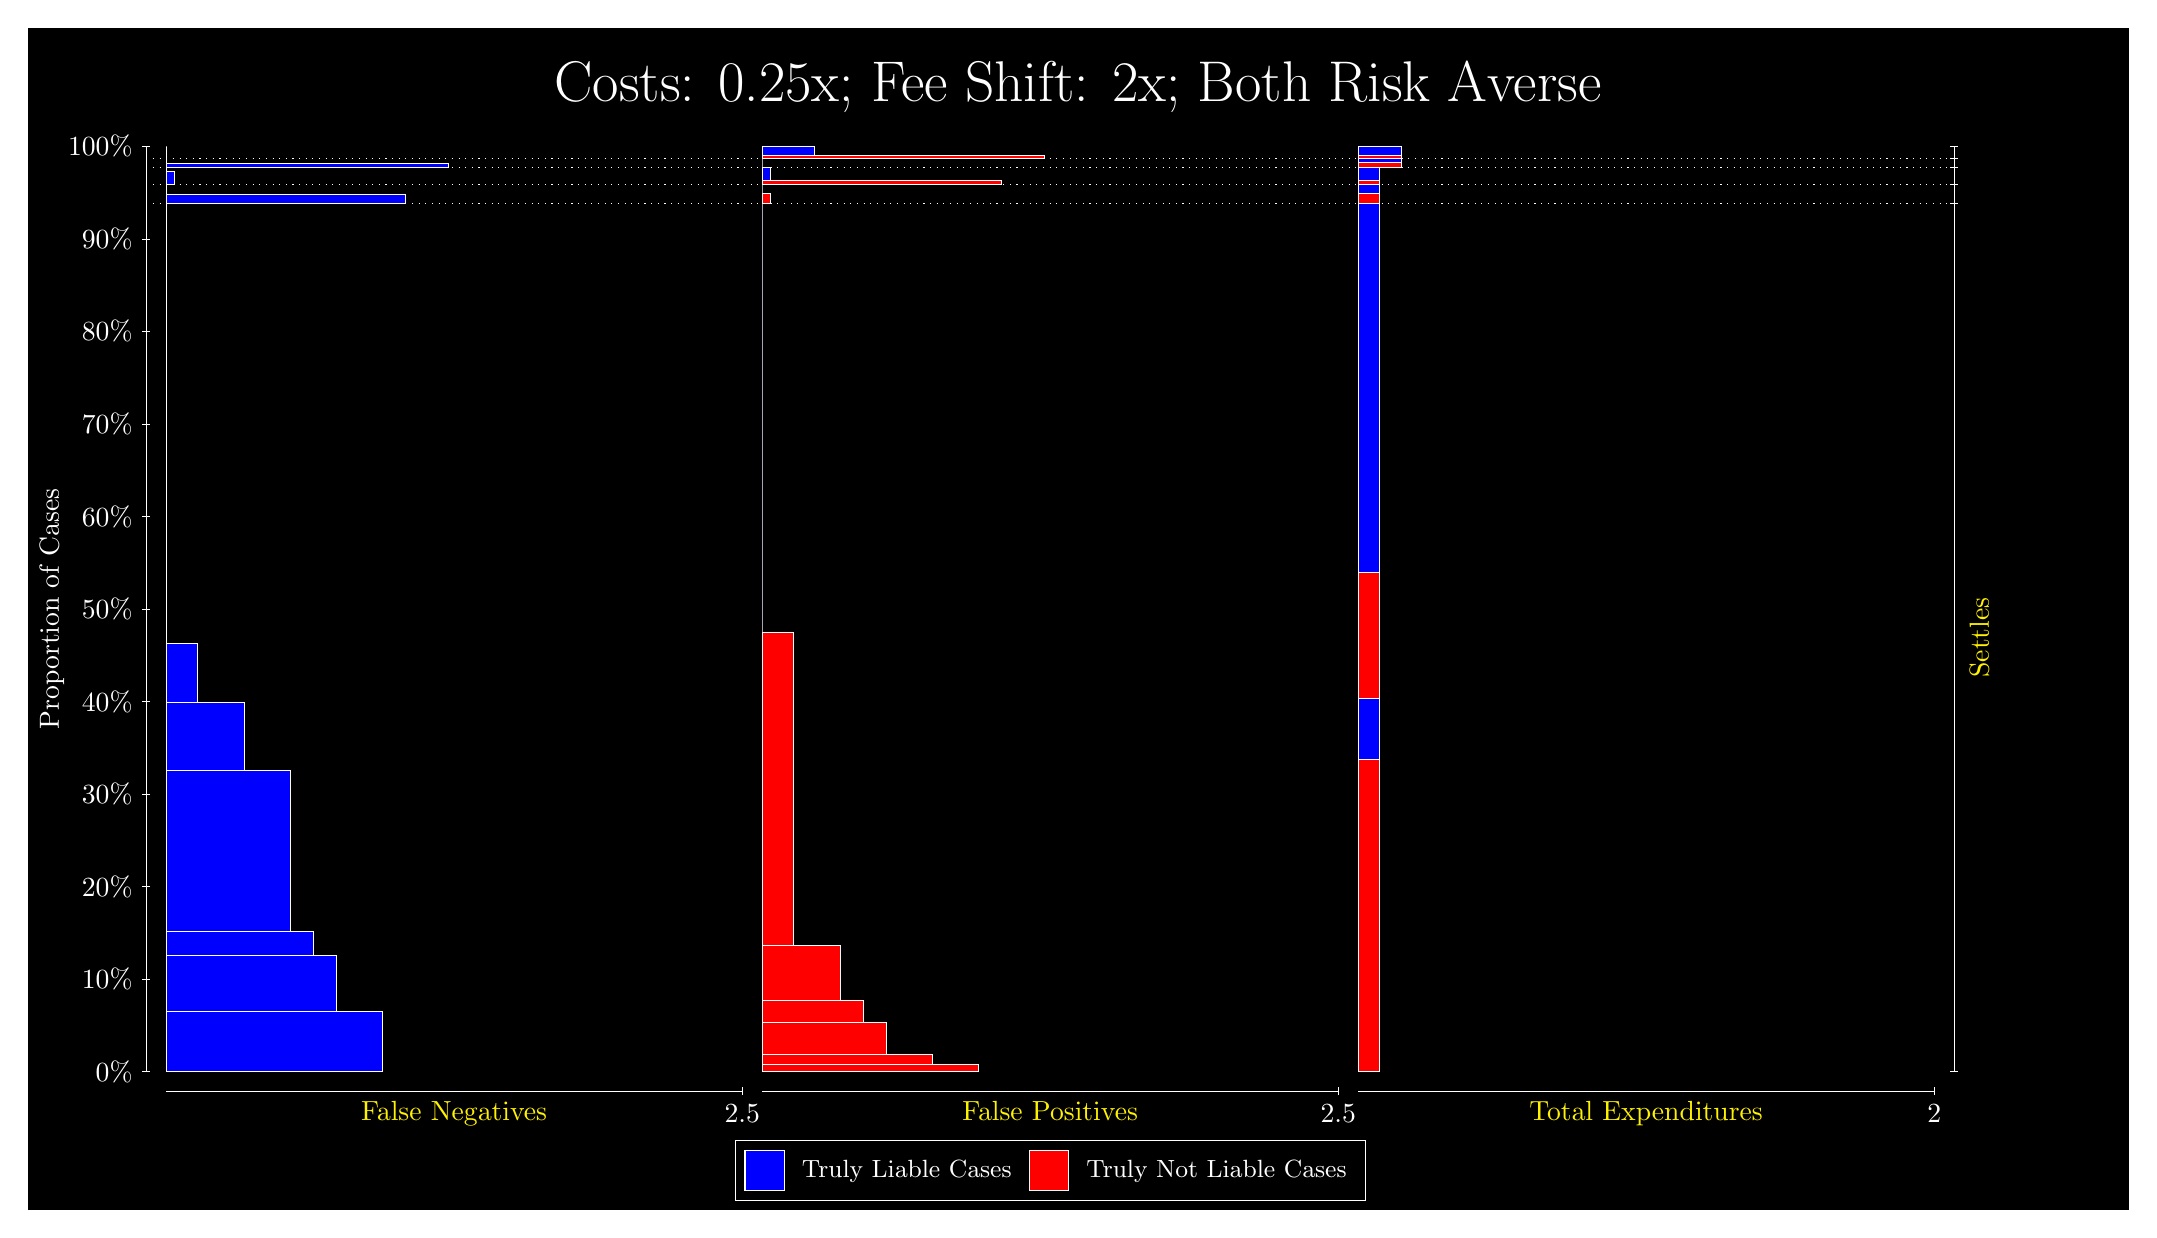
\begin{tikzpicture}
\draw[fill=black] (0,0) rectangle (26.667,15);
\draw[text=white] (0,13.5) rectangle (26.667,15) node[midway] {\huge Costs: 0.25x; Fee Shift: 2x; Both Risk Averse};
\draw[white, very thin] (1.5,1.75) -- (1.5,13.5);
\node[rotate=90, text=white, anchor=center] at (0.3, 7.625) {Proportion of Cases};
\draw[white, very thin] (1.45,1.75) -- (1.55,1.75);
\node[text=white, anchor=east] at (1.45, 1.75) {0\%};
\draw[white, very thin] (1.45,2.925) -- (1.55,2.925);
\node[text=white, anchor=east] at (1.45, 2.925) {10\%};
\draw[white, very thin] (1.45,4.1) -- (1.55,4.1);
\node[text=white, anchor=east] at (1.45, 4.1) {20\%};
\draw[white, very thin] (1.45,5.275) -- (1.55,5.275);
\node[text=white, anchor=east] at (1.45, 5.275) {30\%};
\draw[white, very thin] (1.45,6.45) -- (1.55,6.45);
\node[text=white, anchor=east] at (1.45, 6.45) {40\%};
\draw[white, very thin] (1.45,7.625) -- (1.55,7.625);
\node[text=white, anchor=east] at (1.45, 7.625) {50\%};
\draw[white, very thin] (1.45,8.8) -- (1.55,8.8);
\node[text=white, anchor=east] at (1.45, 8.8) {60\%};
\draw[white, very thin] (1.45,9.975) -- (1.55,9.975);
\node[text=white, anchor=east] at (1.45, 9.975) {70\%};
\draw[white, very thin] (1.45,11.15) -- (1.55,11.15);
\node[text=white, anchor=east] at (1.45, 11.15) {80\%};
\draw[white, very thin] (1.45,12.325) -- (1.55,12.325);
\node[text=white, anchor=east] at (1.45, 12.325) {90\%};
\draw[white, very thin] (1.45,13.5) -- (1.55,13.5);
\node[text=white, anchor=east] at (1.45, 13.5) {100\%};

\draw[white, very thin] (24.457,1.75) -- (24.457,13.5);
\draw[white, very thin] (24.407,1.75) -- (24.507,1.75);
\node[anchor=west] at (24.407, 1.75) {};
\draw[white, very thin] (24.407,12.773) -- (24.507,12.773);
\node[anchor=west] at (24.407, 12.773) {};
\draw[white, very thin] (24.407,13.016) -- (24.507,13.016);
\node[anchor=west] at (24.407, 13.016) {};
\draw[white, very thin] (24.407,13.234) -- (24.507,13.234);
\node[anchor=west] at (24.407, 13.234) {};
\draw[white, very thin] (24.407,13.345) -- (24.507,13.345);
\node[anchor=west] at (24.407, 13.345) {};
\draw[white, very thin] (24.407,13.5) -- (24.507,13.5);
\node[anchor=west] at (24.407, 13.5) {};

\draw[white, very thin, fill=blue] (1.75,1.75) rectangle (4.4946,2.5138);
\draw[white, very thin, fill=blue] (1.75,2.5138) rectangle (3.9091,3.2206);
\draw[white, very thin, fill=blue] (1.75,3.2206) rectangle (3.6163,3.532);
\draw[white, very thin, fill=blue] (1.75,3.532) rectangle (3.3236,5.5767);
\draw[white, very thin, fill=blue] (1.75,5.5767) rectangle (2.738,6.4407);
\draw[white, very thin, fill=blue] (1.75,6.4407) rectangle (2.1525,7.1926);
\draw[white, very thin, fill=red] (1.75,7.1926) rectangle (1.75,12.773);
\draw[white, very thin, fill=blue] (1.75,12.773) rectangle (4.7873,12.888);
\draw[white, very thin, fill=red] (1.75,12.888) rectangle (1.75,13.016);
\draw[white, very thin, fill=blue] (1.75,13.016) rectangle (1.8598,13.178);
\draw[white, very thin, fill=red] (1.75,13.178) rectangle (1.75,13.234);
\draw[white, very thin, fill=blue] (1.75,13.234) rectangle (5.3362,13.279);
\draw[white, very thin, fill=red] (1.75,13.279) rectangle (1.75,13.345);
\draw[white, very thin, fill=red] (1.75,13.345) rectangle (1.75,13.389);
\draw[white, very thin, fill=blue] (1.75,13.389) rectangle (1.75,13.5);
\draw[white, very thin, fill=red] (9.3189,1.75) rectangle (12.063,1.8396);
\draw[white, very thin, fill=red] (9.3189,1.8396) rectangle (11.478,1.9684);
\draw[white, very thin, fill=red] (9.3189,1.9684) rectangle (10.892,2.373);
\draw[white, very thin, fill=red] (9.3189,2.373) rectangle (10.6,2.652);
\draw[white, very thin, fill=red] (9.3189,2.652) rectangle (10.307,3.3589);
\draw[white, very thin, fill=red] (9.3189,3.3589) rectangle (9.7214,7.3303);
\draw[white, very thin, fill=blue] (9.3189,7.3303) rectangle (9.3189,12.773);
\draw[white, very thin, fill=red] (9.3189,12.773) rectangle (9.4287,12.9);
\draw[white, very thin, fill=blue] (9.3189,12.9) rectangle (9.3189,13.016);
\draw[white, very thin, fill=red] (9.3189,13.016) rectangle (12.356,13.072);
\draw[white, very thin, fill=blue] (9.3189,13.072) rectangle (9.4287,13.234);
\draw[white, very thin, fill=red] (9.3189,13.234) rectangle (9.3189,13.301);
\draw[white, very thin, fill=blue] (9.3189,13.301) rectangle (9.3189,13.345);
\draw[white, very thin, fill=red] (9.3189,13.345) rectangle (12.905,13.389);
\draw[white, very thin, fill=blue] (9.3189,13.389) rectangle (9.9776,13.5);
\draw[white, very thin, fill=red] (16.888,1.75) rectangle (17.162,5.7215);
\draw[white, very thin, fill=blue] (16.888,5.7215) rectangle (17.162,6.4853);
\draw[white, very thin, fill=red] (16.888,6.4853) rectangle (17.162,8.0941);
\draw[white, very thin, fill=blue] (16.888,8.0941) rectangle (17.162,12.773);
\draw[white, very thin, fill=red] (16.888,12.773) rectangle (17.162,12.9);
\draw[white, very thin, fill=blue] (16.888,12.9) rectangle (17.162,13.016);
\draw[white, very thin, fill=red] (16.888,13.016) rectangle (17.162,13.072);
\draw[white, very thin, fill=blue] (16.888,13.072) rectangle (17.162,13.234);
\draw[white, very thin, fill=red] (16.888,13.234) rectangle (17.437,13.301);
\draw[white, very thin, fill=blue] (16.888,13.301) rectangle (17.437,13.345);
\draw[white, very thin, fill=red] (16.888,13.345) rectangle (17.437,13.389);
\draw[white, very thin, fill=blue] (16.888,13.389) rectangle (17.437,13.5);
\draw[white, dotted] (1.5,12.773) -- (24.457,12.773);
\draw[white, dotted] (1.5,13.016) -- (24.457,13.016);
\draw[white, dotted] (1.5,13.234) -- (24.457,13.234);
\draw[white, dotted] (1.5,13.345) -- (24.457,13.345);
\draw[white, very thin] (1.75,1.5) -- (9.0689,1.5);
\node[text=yellow, anchor=north] at (5.4094, 1.5) {False Negatives};
\draw[white, very thin] (9.0689,1.45) -- (9.0689,1.55);
\node[text=white, anchor=north] at (9.0689, 1.45) {2.5};

\draw[white, very thin] (9.3189,1.5) -- (16.638,1.5);
\node[text=yellow, anchor=north] at (12.978, 1.5) {False Positives};
\draw[white, very thin] (16.638,1.45) -- (16.638,1.55);
\node[text=white, anchor=north] at (16.638, 1.45) {2.5};

\draw[white, very thin] (16.888,1.5) -- (24.207,1.5);
\node[text=yellow, anchor=north] at (20.547, 1.5) {Total Expenditures};
\draw[white, very thin] (24.207,1.45) -- (24.207,1.55);
\node[text=white, anchor=north] at (24.207, 1.45) {2};

\node[text=yellow, centered, rotate=90] at (24.777, 7.2615) {Settles};





\draw (12.978300999999998,1.5) node[draw=none] (baseCoordinate) {};
\begin{scope}[align=center]
        \matrix[scale=0.5, draw=white, below=0.5cm of baseCoordinate, nodes={draw}, column sep=0.1cm]{
            \node[rectangle, draw, minimum width=0.5cm, minimum height=0.5cm, fill=blue] {}; &
            \node[draw=none, font=\small, text=white] (B) {Truly Liable Cases}; &
            \node[rectangle, draw, minimum width=0.5cm, minimum height=0.5cm, fill=red] {}; &
            \node[draw=none, font=\small, text=white] (B) {Truly Not Liable Cases}; \\
            };
\end{scope}

\end{tikzpicture}
\end{document}